\newif\ifincludecopyrightedmaterial
\newif\ifwideformat
%--------------------------------------------------------------------------%
\includecopyrightedmaterialtrue
\wideformattrue
%--------------------------------------------------------------------------%
\ifwideformat
\documentclass[aspectratio=196]{slides}
\else
\documentclass{slides}
\fi
%--------------------------------------------------------------------------%
\usepackage{times,mathptm,graphicx,color,xcolor,hyperref,amsfonts}
\usepackage{amsmath}
\usepackage{enumitem,multirow,amsopn,proof,ulem}
\usepackage{algorithm}
\usepackage[noend]{algpseudocode}
\usepackage{wasysym}
\ifwideformat
\usepackage[noheadfoot,paperheight=210mm,paperwidth=373mm,hmargin=1cm,bottom=5pt,top=5pt]{geometry}
\else
\usepackage[noheadfoot,a4paper,landscape,hmargin=1cm,bottom=5pt,top=5pt]{geometry}
\fi
\usepackage[utf8]{inputenc}
\usepackage{multicol}
\usepackage{tikz}
%\usepackage{showframe}
\texorpdfstring{}{}
%--------------------------------------------------------------------------%
\setitemize{itemsep=0pt,topsep=-1ex}
\def\labelitemi{%
  \textcolor{darkgray}{\raisebox{.3ex}{\rule{.8ex}{.8ex}}}\hspace{.5ex}}
\def\labelitemii{%
  \textcolor{gray}{\raisebox{.35ex}{\rule{.7ex}{.7ex}}}\hspace{.5ex}}
\def\labelitemiii{%
  \textcolor{lightgray}{\raisebox{.35ex}{\rule{.7ex}{.7ex}}}\hspace{.5ex}}
\definecolor{lightlightgray}{rgb}{0.90, 0.90, 0.90}
\def\labelitemiv{%
  \textcolor{lightlightgray}{\raisebox{.35ex}{\rule{.7ex}{.7ex}}}\hspace{.5ex}}
%--------------------------------------------------------------------------%
\def\TITLE#1{\hbox to \linewidth{\large #1\hfill}}
\def\BOTTOM{\vfill\newpage}
\def\SLIDE#1{\BOTTOM\TITLE{#1}}
%--------------------------------------------------------------------------%
\definecolor{darkgreen}{rgb}{0,.5,0}
\definecolor{darkred}{rgb}{0.5,0,0}
\definecolor{darkblue}{rgb}{0,0,0.5}
\def\blue{\color{darkblue}}
\def\magenta{\color{darkred}}

%%%%%%%%%%%%%%%%%%%%%%%%%%%%%%%%%%%%%%%%%%%%%%%%%%%%%%%%%%%%%%%%%%%%%%%%%%%%%%
\begin{document}
\begin{center}
{\huge Solving CNF-XOR Formulas: A Practical Perspective} \\[1cm]
{\Large Mate Soos}\\[1cm]

%\includegraphics[width=8cm]{pdfs/jku}
%\\[1cm]
{\large Simons Institute SAT Program Seminar}
\\[2ex]
%{\large  IIT Bombay, India} \\[4ex]
22nd of February, 2021 \\[16ex]

%{\large  Based on slides by \textbf{Armin Biere}\\}
\end{center}
\newpage
%%%%%%%%%%%%%%%%%%%%%%%%%%%%%%%%%%%%%%%%%%%%%%%%%%%%%%%%%%%%%%%%%%%%%
\SLIDE{About Me}
\begin{itemize}
\item PhD at INRIA Grenoble 2009
\item Maintainer of CryptoMiniSat, ApproxMC, UniGen, STP
\item Working as a Senior Research Fellow at National University of Singapore (3mo a year)
\item Working as a Senior IT Security Architect at Zalando (9mo a year)
\item Interests: SAT solving, Counting, Sampling, Machine Learning, Higher level abstractions
\end{itemize}
\vfill
\newpage

%%%%%%%%%%%%%%%%%%%%%%%%%%%%%%%%%%%%%%%%%%%%%%%%%%%%%%%%%%%%%%%%%%%%%%%%%%%%
\SLIDE{CNF-XOR}

CNF with XORs occur in a number of problem domains, for example:
\begin{itemize}
\item Cryptography. ex find the key given partially observed circuit data [MohamedBulyginZHW2012]
\item Adder and multiplier circuits: ex. see Daniela Kaufmann's presentation ``Combining SAT and Computer Algebra for Circuit Verification'' (February 16th) [KaufmannBiereKauers2019]
\item Polynomial systems over GF(2): ex.

$\begin{array}{llllllll}
ab &\oplus &b &\oplus &efd &\oplus &e &= 0\\
a &\oplus &e &\oplus &fd &&&= 0\\
abcd &\oplus &e &\oplus &f &&&= 0\\
\end{array}$

See e.g. Bosphorus [ChooSoosChaiMeel19]

\item Hashed-based counting and sampling [ChakrabortyMeelVardi2003]
\end{itemize}

In this talk, we'll use approximate counting as our reference problem

\vfill
\newpage
%%%%%%%%%%%%%%%%%%%%%%%%%%%%%%%%%%%%%%%%%%%%%%%%%%%%%%%%%%%%%%%%%%%%%%%%%%%%
\SLIDE{Motivating Problem: Approximate Counting}

\begin{itemize}
\item ApproxMC by Chakraborty, Meel, and Vardi (2003): A Scalable Approximate Model Counter
\item Random XORs over the projection set: a hashing-based strategy to probably approximately count solutions
\item 99\% of its time is spent in the SAT solver solving CNF-XOR formulas
\end{itemize}

(1) Pick a random cell, (2) count solutions, (3) multiply by no. cells
\begin{center}
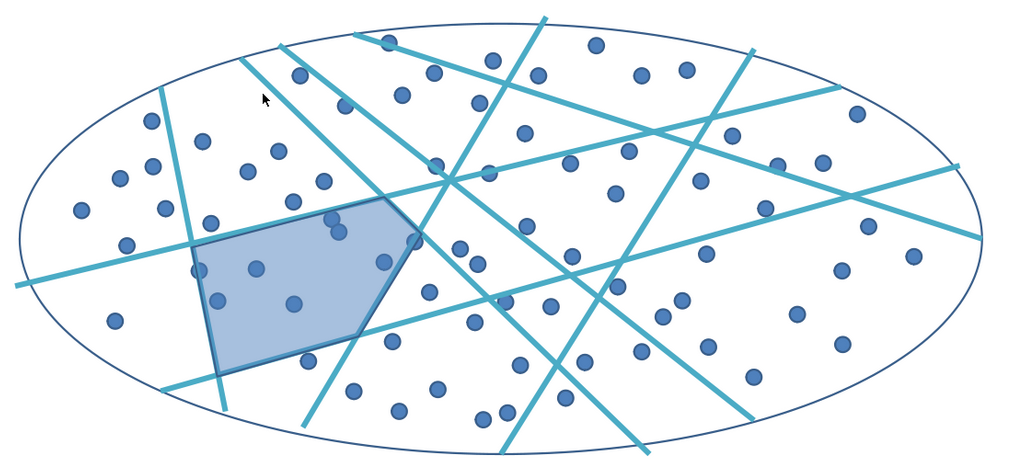
\includegraphics[width=24cm]{cuts_on_plane.png}
\end{center}

\vfill
\newpage


%%%%%%%%%%%%%%%%%%%%%%%%%%%%%%%%%%%%%%%%%%%%%%%%%%%%%%%%%%%%%%%%%%%%%%%%%%%%
\SLIDE{XORs in CNF}

Translating $a\oplus b\oplus c=1$ into CNF using Tseitin transformation [Tseitin'66]:

$\begin{array}{rrrrr}
a& \vee &b& \vee &c\\
a& \vee &\neg b& \vee &\neg c\\
\neg a& \vee &\neg b& \vee &c\\
\neg a& \vee &b& \vee &\neg c\\
\end{array}$

An XOR for size N needs $2^{n-1}$ clauses to translate without helper variables.

To translate an XOR $a\oplus b\oplus c\oplus d\oplus e\oplus f=0$, we cut it into two XORs, using a helper variable {\color{red}x}:

$\begin{array}{lllllll}
a& \oplus &b& \oplus &c & \oplus &{\color{red}x}\\
{\color{red}x}& \oplus &d& \oplus &e & \oplus &f\\
\end{array}$

Using as many helper variables as needed cuts down the blowup to linear size. It increases the number of variables, but that's not really an issue. Modern SAT solvers can deal with millions of variables. However....

\vfill
\newpage

%%%%%%%%%%%%%%%%%%%%%%%%%%%%%%%%%%%%%%%%%%%%%%%%%%%%%%%%%%%%%%%%%%%%%%%%%%%%
\SLIDE{XOR manipulation once in CNF format}

\begin{itemize}
\item XORs can be recovered syntactically and semantically
\item Syntactic recovery seems easy but:

$\begin{array}{rrrrr}
a& \vee &b& \\
a& \vee &\neg b& \vee &\neg c\\
\neg a& \vee &\neg b& \vee &c\\
\neg a& \vee &b& \vee &\neg c\\
\end{array}$
$\rightarrow$ still implies the XOR, so complication arise
\item Once recovered, XORs can be re-assembled:

$\begin{array}{lllllll}
a& \oplus &b& \oplus &c & \oplus &{\color{red}x}\\
{\color{red}x}& \oplus &d& \oplus &e & \oplus &f\\
\end{array}$

becomes

$a\oplus b\oplus c\oplus d\oplus e\oplus f=0$

\item XORs in different matrices can be extracted by grouping XORs together that coincide on at least one variable.

$\rightarrow$ Since naive GJE is O($n^3$), if we have two matrices of n/2 size, we'll be $\approx 4$x faster working on them separately

\item Running GJE on the reassembled XORs is easy, but does not suffice -- it will only perform GJE at ``toplevel'', i.e. without any assignments by the solver.
\end{itemize}


\vfill
\newpage

%%%%%%%%%%%%%%%%%%%%%%%%%%%%%%%%%%%%%%%%%%%%%%%%%%%%%%%%%%%%%%%%%%%%%%%%%%%%%
\SLIDE{Resolution on XOR formulas}

\begin{itemize}
\item Standard (non-extended) resolution is bad at proving UNSAT of XORs blasted into CNF
\item Actually, the minimum size resolution proof can be made to be exponential in the number of variables
\item But naive Gauss-Jordan Elimination (GJE) is only O($n^3$)
\item We need to combine GJE with CDCL or we won't have a hope of solving some of these formulas
\end{itemize}

N.B.: We don't always need GJE just because there are XORs. E.g. if there is an UNSAT core that doesn't contain a single clause from the XORs, it can be OK (though there may be a smaller UNSAT proof with the XORs)


\vfill
\newpage


%%%%%%%%%%%%%%%%%%%%%%%%%%%%%%%%%%%%%%%%%%%%%%%%%%%%%%%%%%%%%%%%%%%%%%%%%%%%
\SLIDE{Gaussian Elimination}

Gaussian elimination [UnknownChineseAuthor(s)179, Newton1670] is an algorithm in linear algebra for solving a system of linear equations. Let's restrict ourselves to linear equations over GF(2), i.e. to:

$\begin{array}{llllll}
x_1 &&&\oplus &x_3 &= 0\\
x_1 &\oplus &x_2 &\oplus &x_3 &= 1\\
x_1 &\oplus &x_2 &&&= 0\\
\end{array}$
$\rightarrow$ In matrix notation:
\begin{minipage}{0.3\linewidth}
\[
\left[
\begin{array}{lll|l}
x_1 & x_2 & x_3 & $RHS$\\
1 &            0 &           1 & 0\\
1 &            1 &           1 & 1\\
1 &            1 &           0 & 0\\
\end{array}
\right]
\]
\end{minipage}

In Gaussian Elimination, we aim to modify the matrix until the lower left-hand corner of the matrix is filled with zeros, also called the \textbf{upper triangular form}:

\begin{minipage}{0.2\linewidth}
\[
\left[
\begin{array}{lll|l}
\color{red}{1} &            0 &           1 & 0\\
1 &            1 &           1 & 1\\
1 &            1 &           0 & 0\\
\end{array}
\right]
\]
\end{minipage}
\begin{minipage}{0.4\linewidth}
$\rightarrow$ XOR row of leftmost ``1'' into all rows where `1'' is present in that column
\end{minipage}
\begin{minipage}{0.2\linewidth}
\[
\left[
\begin{array}{lll|l}
1 &            0 &           1 & 0\\
0 &            1 &           0 & 1\\
0 &            1 &           1 & 0\\
\end{array}
\right]
\]
\end{minipage}

\begin{minipage}{0.2\linewidth}
\[
\left[
\begin{array}{lll|l}
1 &            0 &           1 & 0\\
0 &            \color{red}{1} &           0 & 1\\
0 &            1 &           1 & 0\\
\end{array}
\right]
\]
\end{minipage}
\begin{minipage}{0.4\linewidth}
$\rightarrow$ XOR row of 2nd  leftmost ``1'' into all rows where `1'' is present in that column
\end{minipage}
\begin{minipage}{0.2\linewidth}
\[
\left[
\begin{array}{lll|l}
1 &            0 &           1 & 0\\
0 &            1 &           0 & 1\\
0 &            0 &           1 & 1\\
\end{array}
\right]
\]
\end{minipage}


\vfill
\newpage
%%%%%%%%%%%%%%%%%%%%%%%%%%%%%%%%%%%%%%%%%%%%%%%%%%%%%%%%%%%%%%%%%%%%%%%%%%%%
\SLIDE{Gaussian Elimination cont.}

\begin{minipage}{0.2\linewidth}
\[
\left[
\begin{array}{lll|l}
\color{red}{1} &            0 &           1 & 0\\
1 &            1 &           1 & 1\\
1 &            1 &           0 & 0\\
\end{array}
\right]
\]
\end{minipage}
\begin{minipage}{0.4\linewidth}
$\rightarrow$ XOR row of leftmost ``1'' into all rows where `1'' is present in that column
\end{minipage}
\begin{minipage}{0.2\linewidth}
\[
\left[
\begin{array}{lll|l}
1 &            0 &           1 & 0\\
0 &            1 &           0 & 1\\
0 &            1 &           1 & 0\\
\end{array}
\right]
\]
\end{minipage}

\begin{minipage}{0.2\linewidth}
\[
\left[
\begin{array}{lll|l}
1 &            0 &           1 & 0\\
0 &            \color{red}{1} &           0 & 1\\
0 &            1 &           1 & 0\\
\end{array}
\right]
\]
\end{minipage}
\begin{minipage}{0.4\linewidth}
$\rightarrow$ XOR row of 2nd  leftmost ``1'' into all rows where `1'' is present in that column
\end{minipage}
\begin{minipage}{0.2\linewidth}
\[
\left[
\begin{array}{lll|l}
1 &            0 &           1 & 0\\
0 &            1 &           0 & 1\\
0 &            0 &           1 & 1\\
\end{array}
\right]
\]
\end{minipage}

What if the matrix doesn't look so pretty?

\begin{itemize}
\item We can \textbf{swap rows} to make sure the 1st row has a ``1'' in the leftmost column
\item If a row contains $[000\ldots0|1]$ then the set of linear equations cannot be satisfied, i.e. \textbf{UNSAT}
\item If the matrix is \textbf{underdetermined}, if there is a solution, it's never a single solution. E.g. 20 variables but only 5 equations.
\end{itemize}


\vfill
\newpage

%%%%%%%%%%%%%%%%%%%%%%%%%%%%%%%%%%%%%%%%%%%%%%%%%%%%%%%%%%%%%%%%%%%%%%%%%%%%
\SLIDE{Gauss-Jordan Elimination}
Gauss-Jordan Elimination lets Gaussian Elimination finish, then goes from right to left, bottom to top:


\begin{minipage}{0.2\linewidth}
\[
\left[
\begin{array}{lll|l}
1 &            0 &           1 & 0\\
0 &            1 &           0 & 1\\
0 &            0 &           \color{red}{1} & 1\\
\end{array}
\right]
\]
\end{minipage}
\begin{minipage}{0.4\linewidth}
$\rightarrow$ XOR the row of rightmost ``1'' into all rows above where a ``1'' is present
\end{minipage}
\begin{minipage}{0.2\linewidth}
\[
\left[
\begin{array}{lll|l}
1 &            0 &           0 & 1\\
0 &            1 &           0 & 1\\
0 &            0 &           1 & 1\\
\end{array}
\right]
\]
\end{minipage}

This is known as the \textbf{row echelon form}. We can now trivially read out the solution:

$\begin{array}{ll}
x_1 &= 1\\
x_2 &= 1\\
x_3 &= 1\\
\end{array}$

This indeed satisfies:

$\begin{array}{llllll}
x_1 &&&\oplus &x_3 &= 0\\
x_1 &\oplus &x_2 &\oplus &x_3 &= 1\\
x_1 &\oplus &x_2 &&&= 0\\
\end{array}$


\vfill
\newpage
%%%%%%%%%%%%%%%%%%%%%%%%%%%%%%%%%%%%%%%%%%%%%%%%%%%%%%%%%%%%%%%%%%%%%%%%%%%%
\SLIDE{CDCL(T)}

For theories that are not efficiently simulated by CDCL

\begin{itemize}
\item T is the theory, e.g.:
\begin{itemize}
\item Gauss-Jordan Elimination [SoosNohlCastelluccia'2010]
\item Pseudo-Boolean Reasoning [ChaiKuehlmann'2006]
% Also: Benhamou  and  L.  Granvilliers,  “Continuous  and  Interval  Constraints,”inHandbook  of  Constraint  Programming,  ser.  Foundations  of  ArtificialIntelligence, 2006, pp. 571–603
\item Symmetric Explanation Learning [DevriendtBogaertsBruynooghe'2017]
\end{itemize}
\item Theory is run side-by-side to the CDCL algorithm
\item \textbf{Propagate} values implied by Theory given current assignment stack of CDCL
\item \textbf{Conflict} if Theory implies 1=0 given current assignment stack of CDCL
\item Theory must give reason for propagations\&conflicts
\end{itemize}

\begin{center}
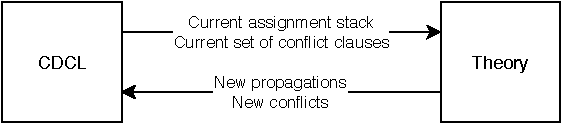
\includegraphics[width=24cm]{CDCL-T}
\end{center}

\vfill
\newpage
%%%%%%%%%%%%%%%%%%%%%%%%%%%%%%%%%%%%%%%%%%%%%%%%%%%%%%%%%%%%%%%%%%%%%%%%%%%%
\SLIDE{CDCL(T) Cont.}

Optimizations:
\begin{itemize}
\item Should only send delta of assignment stack + conflict clauses
\begin{itemize}
\item Variables assigned (decisions + propagations)
\item Variables unassigned (backtracking, restarting)
\item New conflict clauses
\end{itemize}
\item Theory only needs to compute delta relative to old state
\item Theory can give placeholders for reasons
\begin{itemize}
\item If reason is needed during conflict generation, Theory is queried
\item Called ``lazy'' (vs ``greedy'') interpolant generation
\end{itemize}
\end{itemize}
\vspace{2ex}
\begin{center}
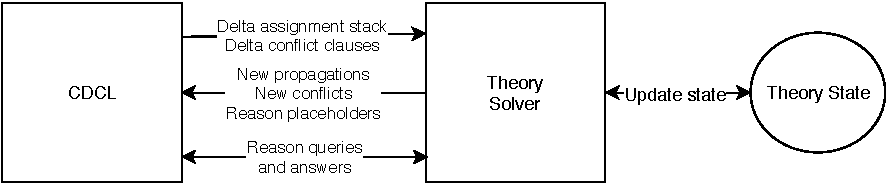
\includegraphics[width=29cm]{CDCL-T-delta}
\end{center}

\vfill
\newpage
%%%%%%%%%%%%%%%%%%%%%%%%%%%%%%%%%%%%%%%%%%%%%%%%%%%%%%%%%%%%%%%%%%%%%%%%%%%%
\SLIDE{CDCL(T) Gauss-Jordan Elimination: Ingredients}

What components do we need?
\begin{itemize}
\item \textbf{Extractor for XOR constraints}: XORs may be encoded as CNF
\item \textbf{Disjoint matrix detection}: disjoint matrices should be handled separately
\item \textbf{Delta update mechanism} for row-echelon form matrix:
\begin{itemize}
    \item how to handle when variable is set
    \item how to handle when variable is unset
\end{itemize}
\item \textbf{Efficient data structures} to allow for quick updates
\item \textbf{Reason generation}
\end{itemize}
\vfill
\newpage

%%%%%%%%%%%%%%%%%%%%%%%%%%%%%%%%%%%%%%%%%%%%%%%%%%%%%%%%%%%%%%%%%%%%%%%%%%%%
\SLIDE{CDCL(T) Gauss-Jordan Elimination: None of that row swapping please!}
\vspace{2ex}

Observations:
\begin{itemize}
\item We are using binary matrices (1/0), so bit-packed format is best
\item Packed format: row-swapping becomes expensive -- it's a copy
\item Row-echelon form is nice for the eyes [HanJiang2012]:
\begin{itemize}
\item But we only need a row to be responsible for a column's ``1''
\item What we loose: have to check all rows, not only ones below
\end{itemize}
\item So, any row can be responsible for being a column's ``1''
\end{itemize}

\begin{center}
\begin{minipage}{0.2\linewidth}
\[
\left[
\begin{array}{llllllll|l}
x_1 & x_2 & x_2 & x_3 & x_4 & x_5 & x_6 & x_7 & $RHS$\\
0 & 0 & 0 & 1 & 1 & 1 & 0 & \color{red}1 & 1\\
1 & \color{red}1 & 0 & 1 & 0 & 1 & 0 & 0 & 1\\
1 &0 &0 & 0 & 0 & 0 & \color{red}1 & 0 & 0\\
1 &0 &\color{red}1 & 1 & 0 & 1 & 0 & 0 & 0\\
\end{array}
\right]
\]
\end{minipage}
\end{center}

The top line reads: $x_3 \oplus x_4 \oplus x_5 \oplus x_7 = 1$



\vfill
\newpage
%%%%%%%%%%%%%%%%%%%%%%%%%%%%%%%%%%%%%%%%%%%%%%%%%%%%%%%%%%%%%%%%%%%%%%%%%%%%
\SLIDE{CDCL(T) Gauss-Jordan Elimination: 2-variable watchlist scheme}
\vspace{2ex}

Let's use a 2-variable watch scheme [HanJiang2012]:
\begin{itemize}
\item If 2 or more variables are unset in XOR constraint, it cannot propagate or conflict
\item If 1 variable is unset, it must propagate
\item If 0 variable is unset, it is either satisfied or is in conflict
\end{itemize}

We'll use the Simplex Method's terminology [Danzig'82]:
\begin{itemize}
\item Let's call the column that the row is responsible for ``{\color{red}basic}''
\item Let's call the column that the row is NOT responsible for ``nonbasic''
\end{itemize}

What data structures do we need for this? Let's see:
\begin{itemize}
\item Watchlist for variables (not literals!)
\item column-has-responsible-row[column] = 1/0
\item row-to-nonbasic-column[row] = column
\end{itemize}
\vfill
\newpage
%%%%%%%%%%%%%%%%%%%%%%%%%%%%%%%%%%%%%%%%%%%%%%%%%%%%%%%%%%%%%%%%%%%%%%%%%%%%
\SLIDE{CDCL(T) Gauss-Jordan Elimination: Propagation}
\vspace{2ex}

A rough outline:
\begin{itemize}
\item Observe that the matrix is usually underdetermined: more columns than rows
\item Many unset columns will have no responsible rows
\item If we set a variable, its column doesn't need a responsible row
\item The more variables we decide on, the more the matrix will be determined
\end{itemize}

\begin{minipage}{0.3\linewidth}
\[
\left[
\begin{array}{llllllll|l}
0 &            0 &           0 & 1 & 1 & 1 &            0 & \color{red}1 & 1\\
1 & \color{red}1 &           0 & 1 & 0 & 1 &            0 &            0 & 1\\
1 &            0 &           0 & 0 & 0 & 0 & \color{red}1 &            0 & 0\\
1 &            0 &\color{red}1 & 1 & 0 & 1 &            0 &            0 & 0\\
\end{array}
\right]
\]
\end{minipage}
%
\begin{minipage}{0.3\linewidth}
\centering
Let's set the first column to ``1'' $\rightarrow$
\end{minipage}
%
\begin{minipage}{0.3\linewidth}
\[
\left[
\begin{array}{llllllll|l}
\color{darkgreen}0 &            0 &           0 & 1 & 1 & 1 &            0 & \color{red}1 & 1\\
\color{darkgreen}0 & \color{red}1 &           0 & 1 & 0 & 1 &            0 &            0 & 0\\
\color{darkgreen}0 &            0 &           0 & 0 & 0 & 0 & \color{red}1 &            0 & 1\\
\color{darkgreen}0 &            0 &\color{red}1 & 1 & 0 & 1 &            0 &            0 & 1\\
\end{array}
\right]
\]
\end{minipage}

\begin{minipage}{0.3\linewidth}
\centering
we get a propagation!
$\rightarrow$
\end{minipage}
\begin{minipage}{0.3\linewidth}
\[
\left[
\begin{array}{llllllll|l}
\color{darkgreen}0 &            0 &           0 & 1 & 1 & 1 &            0 & 1 & 1\\
\color{darkgreen}0 & 1 &           0 & 1 & 0 & 1 &            0 &            0 & 0\\
\color{darkgreen}0 &            0 &           0 & 0 & 0 & 0 & \color{red}1 &            0 & 1\\
\color{darkgreen}0 &            0 &1 & 1 & 0 & 1 &            0 &            0 & 1\\
\end{array}
\right]
\]
\end{minipage}
\begin{minipage}{0.3\linewidth}
Notice: we were were watching both of this row's variables where it has a ``1''. It's a 2-variable watch scheme!
\end{minipage}


\vfill
\newpage
%%%%%%%%%%%%%%%%%%%%%%%%%%%%%%%%%%%%%%%%%%%%%%%%%%%%%%%%%%%%%%%%%%%%%%%%%%%%
\SLIDE{CDCL(T) Gauss-Jordan Elimination: Propagation}
\vspace{2ex}

\begin{minipage}{0.2\linewidth}
\centering
We got a propagation from last slide:
\end{minipage}
\begin{minipage}{0.3\linewidth}
\[
\left[
\begin{array}{llllllll|l}
\color{darkgreen}0 &            0 &           0 & 1 & 1 & 1 &            0 & 1 & 1\\
\color{darkgreen}0 & 1 &           0 & 1 & 0 & 1 &            0 &            0 & 0\\
\color{darkgreen}0 &            0 &           0 & 0 & 0 & 0 & \color{red}1 &            0 & 1\\
\color{darkgreen}0 &            0 &1 & 1 & 0 & 1 &            0 &            0 & 1\\
\end{array}
\right]
\]
\end{minipage}
%
\begin{minipage}{0.2\linewidth}
\centering
Variable is now set by Gauss-Jordan $\rightarrow$
\end{minipage}
%
\begin{minipage}{0.3\linewidth}
\[
\left[
\begin{array}{llllllll|l}
\color{darkgreen}0 &            0 &           0 & 1 & 1 & 1 & \color{darkgreen}0 & \color{red}1 & 1\\
\color{darkgreen}0 & \color{red}1 &           0 & 1 & 0 & 1 & \color{darkgreen}0 & 0 & 0\\
\color{darkgreen}0 &            0 &           0 & 0 & 0 & 0 & \color{darkgreen}0 & 0 & 0\\
\color{darkgreen}0 &            0 &\color{red}1 & 1 & 0 & 1 & \color{darkgreen}0 & 0 & 1\\
\end{array}
\right]
\]
\end{minipage}

\begin{minipage}{0.2\linewidth}
\centering
Variable is decided on $\rightarrow$
\end{minipage}
\begin{minipage}{0.3\linewidth}
\[
\left[
\begin{array}{llllllll|l}
\color{darkgreen}0 & \color{darkgreen}0 &           0 & 1 & 1 & 1 & \color{darkgreen}0 & \color{red}1 & 1\\
\color{darkgreen}0 & \color{darkgreen}0 &           0 & 1 & 0 & 1 & \color{darkgreen}0 & 0 & 0\\
\color{darkgreen}0 & \color{darkgreen}0 &           0 & 0 & 0 & 0 & \color{darkgreen}0 & 0 & 0\\
\color{darkgreen}0 & \color{darkgreen}0 &\color{red}1 & 1 & 0 & 1 & \color{darkgreen}0 & 0 & 1\\
\end{array}
\right]
\]
\end{minipage}
%
\begin{minipage}{0.2\linewidth}
\centering
Need new basic variable

$\rightarrow$
\end{minipage}
%
\begin{minipage}{0.3\linewidth}
\[
\left[
\begin{array}{llllllll|l}
\color{darkgreen}0 & \color{darkgreen}0 &           0 & 1 & 1 & 1 & \color{darkgreen}0 & \color{red}1 & 1\\
\color{darkgreen}0 & \color{darkgreen}0 &           0 & \color{red}1 & 0 & 1 & \color{darkgreen}0 & 0 & 0\\
\color{darkgreen}0 & \color{darkgreen}0 &           0 & 0 & 0 & 0 & \color{darkgreen}0 & 0 & 0\\
\color{darkgreen}0 & \color{darkgreen}0 &\color{red}1 & 1 & 0 & 1 & \color{darkgreen}0 & 0 & 1\\
\end{array}
\right]
\]
\end{minipage}

\begin{minipage}{0.2\linewidth}
\centering
Must adjust matrix

$\rightarrow$
\end{minipage}
\begin{minipage}{0.3\linewidth}
\[
\left[
\begin{array}{llllllll|l}
\color{darkgreen}0 & \color{darkgreen}0 &           0 &            0 & 1 & 0 & \color{darkgreen}0 & \color{red}1 & 1\\
\color{darkgreen}0 & \color{darkgreen}0 &           0 & \color{red}1 & 0 & 1 & \color{darkgreen}0 &            0 & 0\\
\color{darkgreen}0 & \color{darkgreen}0 &           0 &            0 & 0 & 0 & \color{darkgreen}0 &            0 & 0\\
\color{darkgreen}0 & \color{darkgreen}0 &\color{red}1 &            0 & 0 & 0 & \color{darkgreen}0 &            0 & 1\\
\end{array}
\right]
\]
\end{minipage}
\begin{minipage}{0.2\linewidth}
\centering
New propagation

$\rightarrow$
\end{minipage}
\begin{minipage}{0.3\linewidth}
\[
\left[
\begin{array}{llllllll|l}
\color{darkgreen}0 & \color{darkgreen}0 &\color{darkgreen}0 &            0 & 1 & 0 & \color{darkgreen}0 & \color{red}1 & 1\\
\color{darkgreen}0 & \color{darkgreen}0 &\color{darkgreen}0 & \color{red}1 & 0 & 1 & \color{darkgreen}0 &            0 & 0\\
\color{darkgreen}0 & \color{darkgreen}0 &\color{darkgreen}0 &            0 & 0 & 0 & \color{darkgreen}0 &            0 & 0\\
\color{darkgreen}0 & \color{darkgreen}0 &\color{darkgreen}0 &            0 & 0 & 0 & \color{darkgreen}0 &            0 & 0\\
\end{array}
\right]
\]
\end{minipage}

And the story goes on...

\vfill
\newpage
%%%%%%%%%%%%%%%%%%%%%%%%%%%%%%%%%%%%%%%%%%%%%%%%%%%%%%%%%%%%%%%%%%%%%%%%%%%%
\SLIDE{CDCL(T) Gauss-Jordan Elimination: Reason Clauses}
\vspace{2ex}

What combination of XOR constraints gave us the propagation?
\begin{itemize}
\item The above set of matrices cannot give us the reason clause
\item Easy solution: the ``green'' columns are actually not zeroed out
\item When looking for propagations/conflicts, we check if columns' variable is set. If yes, we pretend it's a 0
\item When looking for reasons, we use the actual values
\item All the row-XOR operations happen as before
\end{itemize}

Hence:
\begin{itemize}
\item Each row is a combination of input XOR constraints
\item It is guaranteed to propagate/conflict under current variable assignment
\end{itemize}

When a variable is set, we are just wearing \textbf{``green glasses'', a bitmask}

\vfill
\newpage
%%%%%%%%%%%%%%%%%%%%%%%%%%%%%%%%%%%%%%%%%%%%%%%%%%%%%%%%%%%%%%%%%%%%%%%%%%%%
\SLIDE{CDCL(T) Gauss-Jordan Elimination: Backtracking}
\vspace{2ex}


If we don't zero out the columns, we get a free bonus! If we need to unset an assignment due to backtracking, we pretend we never set it (remove ``green glasses''):
\begin{itemize}
\item All previous invariants still hold
\item If the column had a responsible row, it still has it
\item Both watches of the row are still good and in the watchlists
\item Matrix looks differently than when we last had this assignment... is that a problem?
\item No! Observe: new matrix could have been reached from the starting position, pivoting differently(!)
\end{itemize}
\vfill
\newpage
%%%%%%%%%%%%%%%%%%%%%%%%%%%%%%%%%%%%%%%%%%%%%%%%%%%%%%%%%%%%%%%%%%%%%%%%%%%%
\SLIDE{CDCL(T) Gauss-Jordan Elimination: Recap}
\vspace{2ex}

Let's recap! What was hard:
\begin{itemize}
\item Extracting XOR constraints
\item Keeping CDCL and GJ in sync:
\begin{itemize}
\item Fast update for variable setting (propagation)
\item Fast update for backtracking (conflict)
\end{itemize}
\item Fast checking for propagation/conflict
\item Lazy reason clause generation
\end{itemize}

\vfill
\newpage
%%%%%%%%%%%%%%%%%%%%%%%%%%%%%%%%%%%%%%%%%%%%%%%%%%%%%%%%%%%%%%%%%%%%%%%%%%%%
\SLIDE{Thank you!}
\vspace{2ex}

\begin{center}
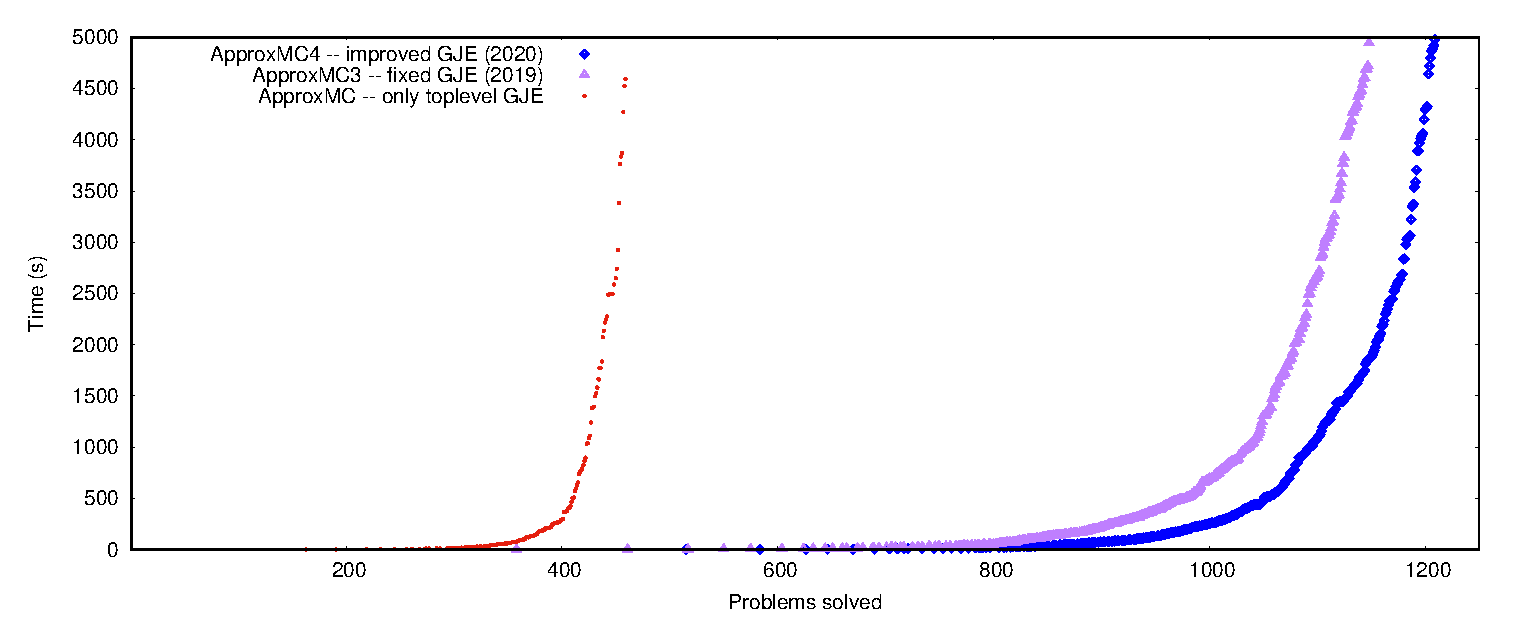
\includegraphics[scale=1.4]{appmc-mate-presentation}
\end{center}

\vfill
\newpage
\end{document}

